\selectlanguage{greek}
\chapter{Εισαγωγή}
\section{Τί είναι τα Συστήματα Εντοπισμού Θέσης}
Τα συστήματα εντοπισμού θέσης (\te{localization systems}) είναι συστήματα
που έχουν τον γενικό στόχο να υπολογίσουν την θέση ενός αντικειμένου μέσα σε έναν δεδομένο χώρο.

Οι διάφορες περιπτώσεις χρήσης αυτών των συστημάτων διαφέρουν σε πολλές παραμέτρους, και για αυτόν τον λόγο τα συστήματα αυτά σχεδιάζονται
για να δουλεύουν εντός κάποιων περιορισμών. Για παράδειγμα το σφάλμα του γνωστού \te{GPS} μπορεί να φτάσει εώς και τα δεκαπέντε μέτρα\cite{acosta}. Μια τέτοια ακρίβεια μπορεί να είναι αποδεκτή σε εφαρμογές εξωτερικών χώρων, αλλά σε καμία περίπτωση δεν είναι αρκετή για μια περίπτωση δωματίου που έχει μήκος ή πλάτος δεκαπέντε μέτρα.

\begin{figure}[h]
\centering
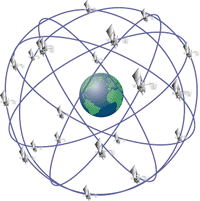
\includegraphics[width=4cm]{pictures/GPS_sat.png}
\caption{Δορυφόροι \te{GPS} \cite{GPS_wikimedia}}
\end{figure}
Απο τήν άλλη, ένα σύστημα εντοπισμού εσωτερικού χώρου μπορεί να προσφέρει ακρίβεια κάτω του ενός μέτρου αλλά η χρήση του περιορίζεται σε έναν σχετικά μικρό χώρο.
\section{Χρησιμότητα του Εντοπισμού θέσης}
Η χρησιμότητα αποδοτικών και εύχρηστων συστημάτων εντοπισμού υψηλής ακρίβειας είναι σχεδόν προφανής. H μοντέρνη καθημερινότητα μας βασίζεται στην χρήση του \te{GPS} κατα την οδήγηση, στις τεχνολογίες \te{Internet of Things}, στην ταχύτατη μεταφορά εμπορευμάτων και αγαθών, στις παροχές έκτακτης ανάγκης και πολλά άλλα.

Είναι λογικό πως για να λειτουργήσουν σωστά όλες αυτές οι υπηρεσίες χρειάζονται τεχνολογίες εντοπισμού οι οποίες είναι προσιτές, δηλαδή δεν έχουν ανάγκη βαρή ή ακριβό υλικό αλλά μπορούν να δουλέψουν με απλές συσκευές όπως το κινητό τηλέφωνο. Να είναι ακριβείς, δηλαδή να προσφέρουν αποδεκτά αποτελέσματα για την κάθε περίπτωση χρήσης και εν τέλη να είναι φθηνές, ωστε να μην μας επιβαρύνουν οικονομικά κατα την καθημερινή χρήση.

Παρακάτω αναφέρουμε μερικά παραδείγματα περιπτώσεων χρήσης τέτοιων συστημάτων.
\subsection{Εντοπισμός Εσωτερικού Χώρου}
\subsubsection{Αποθήκες}
Μια σύγχρονη τεχνολογία που έφαρμόζεται σε μέρη όπως οι αποθήκες είναι ο ρομποτικός έλεγχος, όπου ρομπότ είναι υπεύθυνα για την γρήγορη και αποδοτική μεταφορά
εμπορευμάτων μέσα στην αποθήκη.
Στην περίπτωση του ρομποτικού ελέγχου μπορούν να εφαρμοστούν πιο προηγμένες τεχνικές εντοπισμού εσωτερικού χώρου
απο ο,τι τεχνικές μπορούν να εφαρμοστούν, για παράδειγμα, σε ένα απλό κινητό, καθώς δεν υπάρχουν οι ίδιοι τεχνολογικοί και πρακτική περιορισμοί.
Ο έλεγχος των ρομπότ πραγματοποιείται με συστήματα κανόνων τα οποία βασίζονται στην τοποθεσία των ρομπότ μέσα στην αποθήκη \cite{bernard}.
\begin{figure}[h]
\centering
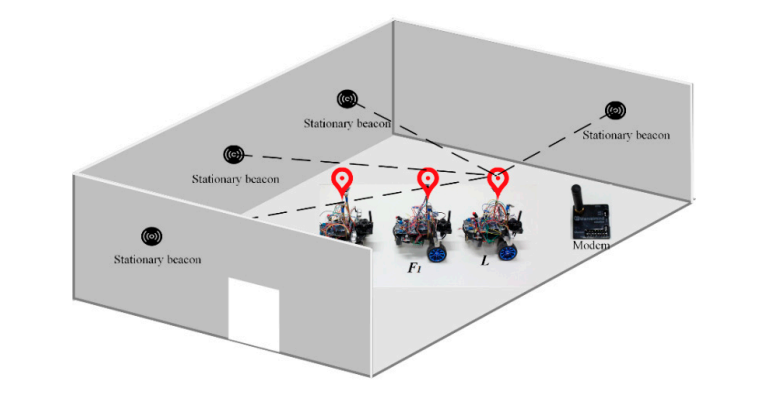
\includegraphics[width=10cm]{pictures/robot_IPS.png}
\caption{Σύστημα Εντοπισμού για Ρομποτικές Εφαρμογές\cite{honganyang}}
\end{figure}

\subsubsection{Πολυκαταστήματα}
Μια άλλη περίπτωση στην οποία τα συστήματα εντοπισμού εφαρμόζονται τα τελευταία χρόνια είναι τα πολυκαταστήματα.
Σε αυτές τις περιπτώσεις όπου υπάρχουν ιδιαίτερεα μεγάλοι και πολύπλοκα διατεταγμένοι χώροι τα συστήματα εντοπισμού βοηθούν τους πελάτες να καθοδηγηθούν μέσα
στον χώρο\cite{spinclabs}. Το κινητό τηλέφωνο του πελάτη ή μια ειδική συσκευή που δίνεται κατα την είσοδο στο κατάστημα χρησιμοποιείται για την εντόπιση του πελάτη
μέσα στο κατάστημα. Έπειτα ο χρήστης μπορεί να καθοδηγηθεί σε διαφορετικούς διαδρόμους ή προϊόντα που τον ενδιαφέρουν, καθώς και σε διάφορα άλλα μέρη όπως για
παράδειγμα χώρους αναψυχής ή εστιατόρια μέσα στο πολυκατάστημα.

\subsubsection{Εποπτεία Ασφαλείας}
Η εποπτεία ασφαλείας είναι μια κατάσταση κατά την οποία ένας άνθρωπος που βρίσκεται απομονωμένος σε κάποιον
χώρο έχει λόγο να νιώθει πως η ασφάλεια του βρίσκεται σε κίνδυνο. Σε αυτήν την περίπτωση κάποιος
υπεύθυνος ασφαλείας μπορεί να ενημερώνεται ανα χρονικά διαστήματα για την τοποθεσία του εν λόγω ανθρώπου μέσο του κινητού
τηλεφώνου του, χρησιμοποιώντας τεχνικές εύρεσης τοποθεσίας.

Σε τέτοιες περιπτώσεις συνήθως υπάρχει και μια λειτουργία έκτακτης ανάγκης, η οποία αμέσως υπολογίζει την τοποθεσία του κινητού τηλεφώνου και την εμφανίζει στον υπεύθηνο ασφαλείας\cite{bernard}.

\subsection{Εντοπισμός Εξωτερικού Χώορυ}
\subsubsection{Πλοήγηση}
Η ιστορικά πρώτη και πιο προφανής εφαρμογή του εντοπισμού εξωτερικού χώρου είναι η πλοήγηση. Εδώ και πολλά χρόνια πλοία και αεροπλάνα χρησιμοποιούν συστήματα όπως το
\te{GPS} για να κατευθυνθούν στην θάλασσα και στον αέρα. Η αλλαγή αυτή ήταν ένα τεράστιο άλμα στην ασφάλεια των ταξιδιών, καθώς αντικατέστησε παλαιότερες μεθόδους
οι οποίες κατα καιρούς είχαν προκαλέσει πολλά ατυχήματα.
Πλέον δεν χρησιμοποιούν μόνο τα πλοία και τα αεροπλάνα το σύστημα \te{GPS} αλλά και φορτηγά και αυτοκίνητα για να κινηθούν σε άγνωστους δρόμους.
\subsubsection{Προσβασιμότητα}
Τα τελευταία χρόνια έχουν αναπτυχθεί συστήματα τα οποία προσπαθούν να βοηθήσουν ανθρώπους με αναπηρίες. Ένα απο αυτά είναι το σύστημα \te{BlindSquare} το οποίο
έχει σκοπό να βοηθάει ανθρώπους με οπτικές αδυναμίες ή αναπηρίες. Το σύστημα αυτό χρησιμοποεί το \te{GPS} για να βοηθήσει αυτούς τους ανθρώπους στην καθοδήγηση τους.
Πιο συγκεκριμένα το \te{BlindSquare} χρησιμοποιεί το κινητό τηλέφωνο του χρήστη και με ακουστικό τρόπο του δίνει πληροφορίες σχετικά με δρόμους, διασταυρώσεις
και κομβικά σημεία\cite{bernard}.
